\documentclass[../../diss.tex]{subfiles}
\begin{document}

\section{\texorpdfstring{$\omega$}{Omega}-regular inclusion}%
\label{Section:EDSOmegaRegIncl}%

In this section, our goal is to extend the results in the previous section from finite to infinite words.
This means we apply effective denotational semantics to the problem of deciding $\omega$-regular inclusion for $\omega$-context-free languages, demonstrating the versatility of the approach.
In contrast to the previous section, this section contains contributions by the author of this thesis.
The content is taken from the publication~\cite{MeyerMN17a}.

\paragraph{$\omega$-regular inclusion}

Formally, the problem that we aim to solve is the following.

\begin{problem}
    \problemtitle{$\omega$-regular inclusion for $\omega$-context-free languages}
    \problemshort{($\OCFLINOREG$)}
    \probleminput{Context-free grammar $G$, NBA $A$.}
    \problemquestion{Does $\olang{G} \subseteq \olang{A}$ hold?}
\end{problem}

In the previous section, we have argued that the problem $\CFLINREG$ corresponds to the verification of the terminating executions of a recursive program.
Similarly, $\OCFLINOREG$ corresponds to verifying the non-terminating executions.

Let us recall the definition of the $\omega$-context-free language $\olang{G}$.
We base our explanation on the techniques that we have developed in the context of the proof of the characterization of $\omega$-context-free languages, \cref{Theorem:CFGOmegaLangCharacterization}.
A word $w \in \Sigma^\omega$ in $\olang{G}$ is obtained from a left-derivation process that can be split into two parts:
The first is an infinite chain of left-derivations of the form $X_i \leftderive \itr{\eta}{i} X_{i+1}$ for all $i \in \N$, where $X_0 = S$ is the initial symbol.
The second part is a collection of finite left-derivation processes $\itr{\eta}{i} \leftderive^* \itr{w}{i}$ for all $i \in \N$ so that $w = \itr{w}{0} \itr{w}{1} \ldots$
To make this formal, we have introduced the spinal graph $\SpinalGraph$ of a grammar in \cref{Section:CFGOmega}, a finite graph whose nodes correspond to nonterminals and whose set of labels is a finite collection of sentential forms.
In $\SpinalGraph$, we have $X \tow{\eta} Y$ iff $X \to \eta.Y$ is a rule of the grammar.
Additionally, we have defined $\calL_G (X)$ to be the language of finite words of the grammar $G$ with the initial symbol replaced by $X$.
We have extended the definition to finite and infinite sentential forms by setting $\calL_G(a) = \set{a}$ for $a \in \Sigma \cup \set{\eps}$ and $\calL_G(\beta_0.\beta_1\ldots) = \calL_G(\beta_1).\calL_G(\beta_2)\ldots$
In \cref{Lemma:CFGOmegaLangSpinalGraph}, we have argued that $\olang{G}$ is exactly the set of infinite words in some $\calL_G(\beta)$, where $\beta \in {(N \cup \Sigma)}^\omega$ is the concatenation of the labels along an infinite path in the spinal graph that starts in $S$.

Our goal is to construct a system of inequalities whose least solutions provides information about both parts of the derivation process as described above.
To handle the finite derivation processes of the shape $\itr{\eta}{i} \leftderive^* \itr{w}{i}$, we proceed as in the previous section.
For each nonterminal $X$ of the grammar, we introduce a variable of the same name, and each production rule $X \to \eta$ induces an inequality
\(
    X \geq \eta
    % \ .
\).
The only difference to the previous section is that we will solve this system using the powerset lattice over the transition monoid of $A$ seen as Büchi automaton (as introduced in \cref{Section:TransitionMonoid}).

Capturing the infinite executions directly is difficult.
We circumvent this problem by using the fact that the behavior of derivation processes for $\olang{G}$ is periodic in a sense that we will make precise later.
For each pair of nonterminals $X,Y$, we add a fresh variable $\cvar{X}{Y}$.
Intuitively, the least solution for $\cvar{X}{Y}$ should represent all finite sentential forms $\beta$ so that $X \leftderive^* \beta.Y$.
To get a finite representation, we do not store $\beta$, but the set of all boxes $\tbox{w}$ where $w$ is a finite word that can be obtained from $\beta$.
Note that $X \leftderive^* \beta.Y$ means that $\beta$ is the concatenation of the labels along a finite path from $X$ to $Y$ in the spinal graph.
Hence, we may use the spinal graph to define the second part of inequalities as follows.

For each edge $X \tow{\eta} Z$ in the spinal graph associated to the given grammar and each nonterminal $Y$, we have an inequality
\[
    \cvar{X}{Y} \geq \eta . \cvar{Z}{Y}
    \ .
\]
Additionally, for each nonterminal $X$, there is the inequality
\[
    \cvar{X}{X} \geq \eps
    \ .
\]
Intuitively, the first inequality states that if we want to get from nonterminal $X$ to the nonterminal $Y$ in the spinal graph and there is a transition $X \tow{\eta} Z$, we can take this transition.
The remaining task is to reach $Y$ from $Z$.
The second inequality states that if we want to reach $X$ from $X$, we can simply stay where we are.


We interpret the whole system of inequalities over $(\powerset{\nbatransmonoid{A}},\subseteq)$, the powerset lattice over the transition monoid of $A$, seen as Büchi automaton.
Terminals $a \in \Sigma$, are interpreted as the singleton set $\set{\tbox{a}}$, the symbol $\eps$ is interpreted as $\set{\tbox{\eps}} = \set{\id}$.
Concatenation is interpreted as the element-wise composition of such sets, $R_1 \comp R_2 = \Set{ \rho_1 \relcomp \rho_2 }{ \rho_1 \in R_1, \rho_2 \in R_2}$.

The powerset lattice over a finite set like $\nbatransmonoid{A}$ satisfies the ACC and the interpretation of all functions is monotonic.
Therefore, we can solve the system of inequalities by applying chaotic iteration.
The following lemma states that the least solution $\sol \colon \vars \to \powerset{\nbatransmonoid{A}}$ indeed has the aforementioned properties.

\begin{lemma}%
\label{Lemma:EDSOmegaRegInclSoundnessHelper}%
    We have $\sol{X} = \Set{ \tbox{w} }{ w \in \calL_G(X)}$ and
    $\sol{\cvar{X}{Y}} = \Set{ \tbox{w} }{ X \leftderive^* \beta.Y, \beta \derive^* w }$\ .
\end{lemma}

The first part of the lemma can be shown exactly as in the proof of \cref{Lemma:EDSRegInclSoundness}.
We conclude that for every finite sentential form $\beta$, $\sol{\beta} = \Set{\tbox{w}}{ w \in \calL_G(\beta)}$.
The second part of the lemma follows using the definition of the spinal graph.
We forgo giving a formal proof.

\paragraph{Representing infinite words}

It remains to use the solution to this system to decide whether the inclusion $\olang{G} \subseteq \olang{A}$ holds.
Before we can explain how to extract this information from the solution, we need to discuss how the behavior of infinite words in a Büchi automaton can be represented by boxes.
In the following, we consider pairs of boxes $(\tau,\rho)$, where $\tau$ describes a finite prefix and $\rho$ describes a behavior that is repeated infinitely.
We write such a pair as $\tau\rho^\omega$, and we define $\lang{\tau\rho^\omega} = \lang{\tau}.\lang{\rho}^\omega$.
The following lemma states that the languages of the shape $\lang{\tau.\rho^\omega}$ cover $\Sigma^\omega$, and that each  $\lang{\tau.\rho^\omega}$ is either completely contained in $\lang{A}$ or disjoint from it.

\begin{lemma}[(\citea{SistlaVW87})]%
\label{Lemma:EDSOmegaRegInclBoxesProperties}%
    \begin{thmenumerate}[a)]
        \item For every $w \in \Sigma^\omega$, there is a pair of boxes $\tau\rho^\omega$ with $w \in \lang{\tau\rho^\omega}$.
        \item For every pair of boxes $\tau\rho^\omega$, we have $\lang{\tau\rho^\omega} \subseteq \olang{A}$ or $\lang{\tau\rho^\omega} \subseteq \overline{\olang{A}}$.
    \end{thmenumerate}
\end{lemma}

To show the first part, one can apply Ramsey's theorem that we will use later to prove the soundness of our algorithm.
The second part follows from the fact that boxes present the behavior of a word in a Büchi automaton.
In particular, they do so in a way that is precise enough to check acceptance.

For us to be able to use this characterization, we need a way to check for a given pair of boxes $\tau \rho^\omega$ whether $\lang{\tau \rho^\omega} \subseteq \olang{A}$.
To this end, we need the notion of a \emph{lasso}, which is modified version of the notion of a \emph{proper language} introduced by \citea{SistlaVW87}.
A lasso in a Büchi automaton is the concatenation of a finite path from the initial state to some state, and a cycle containing that state which is repeated ad infinitum.
To enforce that the word that is read along this infinite path is accepted, the cycle should also contain a final state.
We call a pair of boxes a lasso if each word in its language has a run in the Büchi automaton that is a lasso.
The following definition makes precise how this property can be checked.

\begin{definition}
    A pair of boxes $\tau\rho^\omega$ is a \emph{lasso} if either $\rho = \id$ or if there are sequences of states $q_0,q_1, \ldots, q_p$ and $q_0', \ldots, q_c'$ so that
    (1) $q_0 = \qinit$,
    (2) $\tau(q_0,q_1) > 0$,
    (3) for all $i \in \oneto{p-1}$, $\rho(q_i,q_{i+1}) > 0$,
    (4) $q_p = q_0' = q_c'$,
    (5) for all $j \in \zeroto{c-1}$, $\rho(q_j,q_{j+1}) > 0$, and
    (6) there is $j \in \zeroto{c-1}$ with $\rho(q_j,q_{j+1}) = 2$.
    If $\tau = \id$, we replace the Condition~(2) by requiring $q_0 = q_1$.
\end{definition}

\begin{figure}[t]
    \centering%
    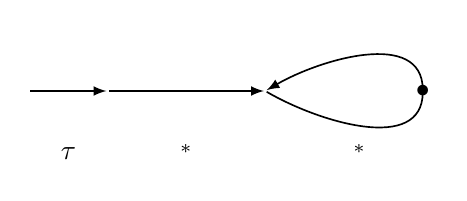
\begin{tikzpicture}[->,>=latex,semithick]

\node (Q0) [inner sep=0em, outer sep=0em] at (0,0) {};
\node (Q1) [inner sep=0em, outer sep=0em] at (1,0) {};
\node (Q2) [inner sep=0em, outer sep=0em] at (3,0) {};
\node (pt) [inner sep=0em, outer sep=0em] at (5,0) {};

\path [draw]
    (Q0) edge (Q1)
    (Q1) edge (Q2)
    (Q2) edge [-, bend right,in=-90] (pt)
    (pt) edge [bend right,out=-90] (Q2)
;
\node at (pt) {$\bullet$};

\node at (0.5,-0.8) {$\tau$};
\node at (2,-0.8) {$\tbox^*$};
\node at (4.2,-0.8) {$\tbox^*$};

\end{tikzpicture}
%
    \caption{A schematic depiction of a lasso $\tau\rho^\omega$, where neither $\tau$ nor $\tbox$ is $\id$. The lasso is a transition in $\tau$, followed by a sequence of transitions in $\tbox$, followed by a cycle of transitions in $\tbox$. One of the transitions along the cycle visits a final state.}%
    \label{Figure:Lasso}
\end{figure}

The definition is visualized in the form of \cref{Figure:Lasso}.
To better understand the definition, it is helpful to see a box $\tbox$ as a directed graph with set of nodes $Q$.
It contains the edge $q \to q'$ iff $\rho(q,q') > 0$.
The first three conditions state that there should be a path leading from the initial state to some state $q_p$ such that the first transition is contained in $\tau$ and all other transitions are contained in $\rho$.
The other conditions require a cycle containing $q_p$ whose transitions are contained in $\rho$.
At least one transition along the cycle is labeled by $2$, meaning that it visits a final state.

This characterization also explains how to check efficiently whether a pair of boxes is a lasso.
It amounts to a polynomial number of reachability checks in directed graphs with $\card{Q}$ nodes, which is a problem that can be solved in polynomial time.

Let us explain why we consider a pair of boxes $\tau\rho^\omega$ with $\tbox = \id$ a lasso.
In this case, we have $\lang{\tau\rho^\omega} = \lang{\tau}.\lang{\rho}^\omega = \lang{\tau}.\set{\eps}^\omega = \lang{\tau}.\emptyset = \emptyset$.
Hence, the inclusion $\lang{\tau\rho^\omega} \subseteq \olang{A}$ holds.

For a pair of boxes that are not equal to $\id$, we also have that the inclusion holds if and only if the language of the pair is included in the language of the NBA.\@
This is because the definition of a lasso mimics the acceptance condition for Büchi automata: Being a lasso means that every word in the associated language has a run that visits a final state infinitely often.
For the formal proof, we would need to invoke \cref{Lemma:EDSOmegaRegInclBoxesProperties}.

Note that here, it is important that we only consider boxes (functions with signature $Q \times Q \to 3$) that actually correspond to elements of the transition monoid, meaning their language is non-empty.
If $\tbox$ or $\tau$ has an empty language, then $\lang{\tau\tbox^\omega}$ is empty and inclusion in $\olang{A}$ trivially holds, no matter whether $\tau\tbox^\omega$ is a lasso.

\begin{lemma}[(\citea{SistlaVW87})]%
\label{Lemma:EDSOmegaRegInclLasso}%
    For boxes $\tbox,\tau$ with non-empty language, $\lang{\tbox} \neq \emptyset \neq \lang{\tau}$, the pair $\tau\rho^\omega$ is a lasso if and only if $\lang{\tau\rho^\omega} \subseteq \olang{A}$.
\end{lemma}

Lassos characterizing whether a pair of boxes represents a language that is either included in or disjoint from the language of an NBA is the final piece we need to solve $\OCFLINOREG$ using effective denotational semantics.
Checking whether the inclusion $\olang{G} \subseteq \olang{A}$ of interest holds amounts to checking whether certain pairs of boxes that are obtained from the least solution to our system of inequalities are lassos.

\begin{theorem}%
\label{Theorem:EDSOmegaRegInclSoundness}%
    The inclusion $\olang{G} \subseteq \olang{A}$ holds if and only if for each nonterminal $X$ and each $\tau \in \sol{\cvar{S}{X}}$, $\rho \in \sol{\cvar{X,X}}$, the pair of boxes $\tau\rho^\omega$ is a lasso.
\end{theorem}

From the theorem, the solution to $\OCFLINOREG$ follows immediately.
We can compute the least solution to the system of inequalities defined before and obtain the sets of boxes $\cvar{S}{X}$ and $\cvar{X}{X}$ for all possible $X$.
It then just remains to check whether all possible pairs of boxes from these sets are lassos.

Before we prove the result, we consider an example.

\begin{example}
    Consider the alphabet $\set{a,r,s,t}$ whose letters should represent the actions of a server.
    Letter $r$ represents that the server has received a request, $a$ represents that it has acknowledged a request, $s$ and $t$ are internal actions.
    A typical liveness property that one would like to verify is that every request gets acknowledged after finite time.
    Unfortunately, this is not an $\omega$-regular property.
    Instead, we consider the simpler property that if the server receives infinitely many requests, it also acknowledges infinitely often.

    The latter property is $\omega$-regular since it is the language of the Büchi automaton $A$ depicted in \cref{Figure:ReqAckNBA}.
    Its set of boxes with non-empty language is depicted in \cref{Figure:ReqAckBoxes}.

    We consider a server whose behavior is described by the $\omega$-context-free language of the grammar with the production rules
    \begin{align*}
        X &\to r Y a \mid XX\ ,
        &Y &\to s Y t \mid \eps\ ,
    \end{align*}
    where $X$ is the initial symbol.
    The language is $\olang{G} = \Set{ {(r (s^{n_i}t^{n_i}) a)}^\omega  }{n_i \in \N \text{ for all } i}$.

    To set up the system of inequalities associated to that grammar, we first observe that its spinal graph consists of the nodes $X$ and $Y$ and the single edge $X \tow{X} X$.
    All transitions but $X \to XX$ are not of the required shape and do not lead to edges in the spinal graph.

    The first part of the system of inequalities for the variables $X$ and $Y$ is the following.
    \begin{align*}
        X &\geq r.Y.a
        &
        Y &\geq s . Y . t
        \\
        X &\geq X.X
        &
        Y &\geq \eps
        \ .
    \end{align*}
    It can be solved independently of the rest, resulting in the least solution $\sol{X} = \set{\tbox{a}}$, $\sol{Y} = \set{\id, \tbox{s}}$.
    The rest of the system of inequalities describes the variables of the shape~$\cvar{-}{-}$:
    \begin{align*}
        \cvar{X}{X} &\geq X.\cvar{X}{X}
        &
        \cvar{X}{Y} &\geq X.\cvar{Y}{X}
        \\
        \cvar{X}{X} &\geq \eps
        &
        \cvar{Y}{Y} &\geq \eps
        \ .
    \end{align*}
    The variable $\cvar{Y}{X}$ has no associated inequality because $Y$ has no outgoing edges in the spinal graph.
    The least solution is $\sol{\cvar{X}{X}} = \set{\id,\tbox{a}}$, $\sol{\cvar{Y}{Y}} = \set{\id}$ and $ \sol{\cvar{X}{Y}} = \sol{\cvar{Y}{X}} = \emptyset$.

    We claim that this solution satisfies the condition in \cref{Theorem:EDSOmegaRegInclSoundness}.
    There are only two non-trivial cases that we have to check, $\id\,\tbox{a}^\omega \in \sol{\cvar{X}{X}} \times \sol{\cvar{X}{X}}$ and $\tbox{a}\tbox{a}^\omega \in \sol{\cvar{X}{X}} \times \sol{\cvar{X}{X}}$.
    We observe that $\tbox{a}$ contains the accepting loop $\tbox{a}(q_0,q_0) = 2$ and that $q_0$ is the initial state, which means that both pairs of boxes form lassos.
    This matches the fact that every word in $\olang{G} = \Set{ {(r (s^{n_i}t^{n_i}) a)}^\omega  }{n_i \in \N \text{ for all } i}$ contains both infinitely many requests and infinitely many acknowledgments.
\end{example}

\begin{figure}[t]
    {\centering\subcaptionbox{Büchi automaton $A$.\label{Figure:ReqAckNBA}}[0.49\textwidth][c]{
        \begin{tikzpicture}[->,>=latex,node distance=7em,semithick]

\node[initial above,state,accepting,above,initial text={}] (A) {$q_0$};
\node[state] (B) [right of=A] {$q_1$};

\path
    (A) edge [bend left ] node [above]  {$r$} (B)
    (B) edge [bend left] node [below] {$a$} (A)
;
\path (A) edge [loop left] node [left] {$a, s, t$} (A);
\path (B) edge [loop right] node [right] {$r, s, t$} (B);

\end{tikzpicture}
}
    }%
    {\centering\subcaptionbox{The boxes of $A$ with non-empty language.\label{Figure:ReqAckBoxes}}[0.49\textwidth][c]{
        \begin{tikzpicture}[>=,->,semithick,scale=0.4]

\pic [] (fid) [transform shape] {tbox={2}{}};
\node [scale=1.5] {$\id$};
\node [below = 1.5em] {$\id = \tbox{\varepsilon}$};

\pic (req) at (3,0) [transform shape] {tbox={2}{1/2/dot, 2/2/}};
\node [below = 1.5em] at (3,0) {$\tbox{r}$};

\pic (ack) at (6,0) [transform shape] {tbox={2}{2/1/dot, 1/1/dot}};
\node [below = 1.5em] at (6,0) {$\tbox{a}$};

\pic (ack) at (9,0) [transform shape] {tbox={2}{1/2/dot, 2/2/dot}};
\node [below = 1.5em] at (9,0) {$\tbox{a.r}$};

\pic (qid) at (12,0) [transform shape] {tbox={2}{1/1/dot,2/2/}};
\node [below = 1.5em] at (12,0) {$\tbox{s} = \tbox{t}$};

\end{tikzpicture}
}
    }%
    \caption{An NBA that checks that infinitely many $r$s implies infinitely many $a$s, and its boxes on the right-hand side. The upper dash on each side of each box $\rho$ represents $q_0$, the lower one represents $q_1$. An undotted edge from $q$ to $p$ stands for $\rho(q,p) = 1$, a dotted edge stands for $\rho(q,p) = 2$, \ie the final state has been visited.}%
    \label{Figure:ReqAck}%
\end{figure}


The rest of this section is dedicated to the proof of \cref{Theorem:EDSOmegaRegInclSoundness}.
One part is straightforward.

\begin{lemma}
    If there is a nonterminal $X$ and boxes $\tau \in \sol{\cvar{S}{X}}$, $\rho \in \sol{\cvar{X,X}}$ such that the pair of boxes $\tau\rho^\omega$ is a not a lasso, the inclusion $\olang{G} \subseteq \olang{A}$ does not hold.
\end{lemma}

\begin{proof}
    Assume that $\tau\rho^\omega$ is not a lasso with $\tau \in \sol{\cvar{S}{X}}$, $\rho \in \sol{\cvar{X,X}}$.
    By \cref{Lemma:EDSOmegaRegInclSoundnessHelper}, there are finite words $v,w$ with $\tbox{v} = \tau$, $\tbox{w} = \rho$
    so that $S \leftderive^* \beta X$, $X \leftderive^* \beta' X$ and $\beta \derive^* v$, $\beta' \derive^* w$.
    Consider the infinite word $v.w^\omega$, which is contained in $\lang{\tau\rho^\omega}$.
    Since $\tau\rho^\omega$ is not a lasso, $\lang{\tau\rho^\omega}$ is not contained in $\olang{A}$ by \cref{Lemma:EDSOmegaRegInclLasso}.
    By Part~b) of \cref{Lemma:EDSOmegaRegInclBoxesProperties}, we have $\lang{\tau\rho^\omega} \subseteq \overline{\olang{A}}$.
    This in particular means that $v.w^\omega \not\in \olang{A}$.
    The definitions of $v$ and $w$ yield an infinite left-derivation process, proving that $v.w^\omega \in \olang{G}$.
    We have obtained $v.w^\omega \in \olang{G} \setminus \olang{A}$,  a counterexample to the inclusion.
\end{proof}

The remaining direction requires more work.
In particular, we have to recall Ramsey's theorem which we will need for the proof.

Ramsey's theorem, a generalization of a result by \citea{Ramsey30}, is an important result from infinitary combinatorics.
It considers undirected complete graphs that are finitely colored, \ie equipped with a function $\lambda \colon E \to C$ that assign to each pair of distinct nodes $v,v' \in V$, $v \neq v'$ one of finitely many colors $\lambda(\set{v,v'}) \in C$ to the corresponding edge $\set{v,v'} \in E$.
The coloring is \emph{monochromatic} if all edges are colored by the same color.

\begin{ntheorem}[Ramsey's theorem]%
\label{Theorem:Ramsey}%
    An infinite finitely colored undirected complete graph always has an infinite monochromatic complete subgraph.
\end{ntheorem}

Ramsey's theorem is standard in the literature, but it seems hard to find a reference that states it in the above form without generalizing it in a way that makes it harder to digest.
To solve this issue, we present a proof.

\begin{proof}
    Let $(V,E)$ be an infinite undirected complete graph and let $\lambda \colon E \to C$ be a finite coloring of its edges.
    Using the well-ordering theorem, we may equip the set of nodes $V$ with some well-order~$\leq$.
    We define an infinite sequence of triples ${\big( V_i,v_i,c_i \big)}_{i \in \N}$ so that
    \begin{itemize}
        \item
            ${(V_i)}_{i \in \N}$ is a descending chain of infinite subsets of $V$, \ie
            $V_0 \supseteq V_1 \supseteq V_2 \supseteq \ldots \,$,
        \item
            each $v_i$ is a node so that $v_{i+1} \in V_i$, and
        \item
            $c_i \in C$ is the color of all edges $\set{v_i,v'}$ for $v' \in V_i$.
    \end{itemize}
    %
    We proceed by induction.
    In the base case, we pick $v_0$ as the least element of $V$ (with respect to the well-order $\leq$) and choose the color $c_0$ and the set $V_0$ so that $V_0 = \Set{ v' \in V }{\lambda(\set{v_0,v'}) = c_0 }$ is infinite.
    Note that such a color has to exist, because the graph contains infinitely many edges of the shape $\set{v_0,v'}$ but $\lambda$ assigns only finitely many distinct colors.
    Also, this choice of $V_0$ and $c_0$ means they indeed have the desired properties.

    Assume we have defined $(V_0,v_0,c_0), \ldots, (V_n,v_n,c_n)$.
    We define $(V_{n+1},v_{n+1},c_{n+1})$ in the following.
    We pick $v_{n+1}$ as the least element of $V_n$, thus satisfying $v_{n+1} \in V_n$.
    We choose $c_{n+1}$ and $V_{n+1}$ so that $V_{n+1} = \Set{ v' \in V_{n} }{\lambda(\set{v_{n+1},v'}) = c_{n+1} }$ is infinite.
    If such a $V_{n+1}$ exists, it obviously is an infinite subset of $V_n$, and it has to exist using the same line of argumentation as before:
    $V_n$ is infinite by induction, so the set of edges $\set{v_{n+1},v'}$ with $v' \in V_n$ is infinite.
    There must be a color that is assigned to infinitely many of these edges by $\lambda$.

    The infinite sequence ${(c_i)}_{i \in \N}$ over the finite set $C$ of colors must contain infinitely many occurrences of some color.
    Pick one such color $c$ and consider the set of the associated nodes $v_i$ so that the color in the triple $(V_i,v_i,c_i)$ equals $c$, $V' = \Set{ v_i }{ c_i = c}$.
    Since $c$ occurs infinitely often in the sequence of the $c_i$, the set $V'$ is infinite.
    We argue that the complete subgraph on the set of nodes $V'$ is monochromatic -- all edges between nodes from $V'$ are colored by $c$.

    Consider two distinct nodes from $V'$ and consider the color of the edge between these two nodes.
    By the definition of $V'$, we may write these nodes as $v_n,v_m$ for some $n,m \in \N$, say with $n < m$.
    This in particular implies $m > 0$, so we have $v_m \in V_{m-1}$.
    The sets $V_i$ form a descending chain, so $n < m$ means that $v_m \in V_n$ holds.
    Now we can use the property of $V_n$ and $c_n$ to obtain that the color of the edge $\set{v_n,v_m}$ is $\lambda(\set{v_n,v_m}) = c_n$.
    The latter equals $c$ since $v_n \in V'$, which is what we wanted to show.
\end{proof}

Ramsey's theorem is needed to prove Part~a) of \cref{Lemma:EDSOmegaRegInclBoxesProperties}, showing that every word in $\Sigma^\omega$ is in the language of some pair of boxes $\tau\tbox^\omega$.
The following proof for the remaining part of \cref{Theorem:EDSOmegaRegInclSoundness} can be seen as an extension of that property.

\begin{lemma}
    If the inclusion $\olang{G} \subseteq \olang{A}$ does not hold, there is a nonterminal $X$ and boxes $\tau \in \sol{\cvar{S}{X}}$, $\rho \in \sol{\cvar{X,X}}$ so that the pair of boxes $\tau\rho^\omega$ is not a lasso.
\end{lemma}

\begin{proof}
    Assume that $w \in \olang{G} \setminus \olang{A}$.
    We use the nature of right-infinite left-derivation processes:
    There is an infinite sequence $X_i \to \itr{\beta}{i} X_{i+1}$ of production rules so that $X_0 = S$ is the initial symbol.
    Furthermore, there is a decomposition of $w = \itr{w}{0}\itr{w}{1}\itr{w}{2} \ldots$ into finite infixes so that $\itr{\beta}{i} \derive^* \itr{w}{i}$ for all $i$.

    Since there are only finitely many nonterminals, there is at least one nonterminal $X$ that appears infinitely often in the sequence of the $X_i$.
    We consider the derivation process for $w$ and merge finite infixes of the above sequence of production rules.
    The result should be a sequence of sentential forms so that
    \[
        S \derive^*
        \itr{v}{0} X
        \derive^*
        \itr{v}{0}\itr{v}{1} X
        \derive^*
        \itr{v}{0}\itr{v}{1}\itr{v}{2}X
        \derive^* \ldots
        \ ,
    \]
    \ie  $w = \itr{v}{0}\itr{v}{1}\itr{v}{2} \ldots$ and each $\itr{v}{i}$ takes us from one occurrence of $X$ as the rightmost symbol of the sentential form to the next one.

    We need to find a pair of boxes $\tau\rho^\omega$ that is not a lasso and whose language contains $w$.
    To this end, we use Ramsey's theorem.
    We construct an undirected complete graph with $\N$ as its set of nodes.
    The graph is finitely colored by assigning a box to each edge.
    For $i < j$, we assign $\lambda(\set{i,j}) = \tbox{\itr{v}{i}.\itr{v}{i+1} \ldots \itr{v}{j-1} }$, the box associated to the infix $\itr{v}{i}.\itr{v}{i+1} \ldots \itr{v}{j-1}$ of $w$.
    By Ramsey's theorem, \cref{Theorem:Ramsey}, this graph has a monochromatic infinite complete subgraph, \ie an infinite subset $M \subseteq \N$ so that there is some box $\rho$ with $\lambda(\set{i,j}) = \rho$ for all $m,m' \in M$, $m \neq m'$.

    We consider a new decomposition of $w$ that is obtained by merging the $\itr{v}{i}$ according to the subset $M$.
    Formally, let $m_0 < m_1 < m_2 < \ldots$ be a strictly ascending sequence that contains exactly the elements of $M$.
    We define
    \[
        \itr{u}{0} = \itr{v}{0} \itr{v}{1} \ldots \itr{v}{m_0 - 1}
        \ , \text{ and}
    \]
    \[
        \itr{u}{i} = \itr{v}{m_i} \itr{v}{m_i + 1} \ldots \itr{v}{m_{i+1} - 1}
    \]
    for $i > 0$.
    Obviously, $w = \itr{u}{0} \itr{u}{1} \itr{u}{2} \ldots$%.
    The first infix $\itr{u}{0}$ is chosen so that it takes us from the initial symbol to an occurrence of $X$ that corresponds to the least element of $M$.
    The other infixes are chosen so that they take us from one occurrence of $X$ to a later one.
    In particular, we have a sequence of left-derivations $S \leftderive^* \itr{\beta}{0}.X$, $X \leftderive^* \itr{\beta}{1}.X$, $\ldots$ so that $\itr{\beta}{i} \derive^* \itr{u}{i}$ for all $i$.

    Consider the pair of boxes $\tau\rho^\omega$, where $\tau = \tbox{\itr{u}{0}}$ is the box associated to $\itr{u}{0}$ and $\rho = \tbox{\itr{u}{1}}$ is the box associated to $\itr{u}{1}$.
    Since the subgraph on $M$ is monochromatic, $\rho$ is the box associated to $\itr{u}{i}$ for all $i > 0$.
    The decomposition $w = \itr{u}{0} \itr{u}{1} \itr{u}{2} \ldots$ is a witness for $w \in \olang{\tau\rho^\omega}$.
    Since $w \not\in \olang{A}$, $\tau\rho^\omega$ cannot be a lasso by \cref{Lemma:EDSOmegaRegInclLasso}.

    To complete the proof, we need to argue that $\tau \in \sol{\cvar{S,X}}$, $\rho \in \sol{\cvar{X}{X}}$.
    With \cref{Lemma:EDSOmegaRegInclSoundnessHelper}, we have $\sol{\cvar{X}{X}} = \Set{ \tbox{u} }{ X \leftderive^* \beta.X, \beta \derive^* u }$.
    We have argued above that $X \leftderive^* \itr{\beta}{i}$ and $\itr{\beta}{i} \derive^* \itr{u}{i}$, so $\rho = \tbox{\itr{u}{i}}$ is indeed contained in $\sol{\cvar{X}{X}}$.
    The reasoning for $\tau \in \sol{\cvar{X,S}}$ is similar.
\end{proof}

With both lemmas proven, the proof of \cref{Theorem:EDSOmegaRegInclSoundness} is complete:
Each of the lemmas shows one of the required implications by contraposition.

\end{document}
